\section{距離センサ}
今回,距離センサとしてPololu VL53L0X Time-of-Flight 距離センサモジュールを採用し,機体の前方に1個,左右に1個ずつの計3個取り付ける.この距離センサモジュールはデジタル$\mathrm{I^{2}C}$インターフェイスを介して距離を測定しており,2.8$\mathrm{[V]}$のリニア・レギュレータと,入力電圧2.6$\mathrm{[V]}$から5.5$\mathrm{[V]}$までに対応する変圧回路を備えている.また,この距離センサモジュールでは赤外線を使用しており,最大2$\mathrm{[m]}$まで計測することができて分解能は1$\mathrm{[mm]}$である.\refig{tof_sensor}にToFセンサの外観を示す.また,以下に仕様を記す\cite{tof_sensor1}.

\begin{itemize}
 \item 動作電圧: 2.6$\mathrm{V}〜5.5\mathrm{V}$
 \item 消費電力: 10$\mathrm{mA}$(通常動作時の平均値)
 \item 検出範囲: 3$\mathrm{cm}〜200\mathrm{cm}$
 \item 重量: 0.5$\mathrm{g}$ (ピンヘッダを除く)
 \item 出力フォーマット$\mathrm{I^{2}C}$: 16ビット読み込み(ミリメートル)
 \item ピンピッチ: 2.54$\mathrm{mm}$ 
\end{itemize}


\subsection{ToF方式}
ToFとはTime-of-Flightの省略形であり,反射光の時間から距離を計算するので,反射光の強度で距離を計測する一般的な測距センサと異なり,測定対象の色や表面状態に依存せずに距離を計測することが可能であり,安定して高フレームレートで測定が可能である\cite{tof_sensor1}.

\begin{figure}[htb]
  \centering
  \includegraphics[width=0.5\hsize]{picture/eps/tof.eps}
  \caption{ToFセンサの外観}
  \label{fig::tof_sensor}
 \end{figure}

\begin{figure}[htb]
  \centering
  \includegraphics[width=0.5\hsize]{picture/eps/tof_experiment_place.eps}
  \caption{ToFセンサの実験装置の外観}
  \label{fig::experiment_place}
\end{figure}

\subsection{$\mathrm{I^{2}C}$}
ここで距離センサモジュールの中で使われている$\mathrm{I^{2}C}$(Inter-Integrated Circuit)について説明する.$\mathrm{I^{2}C}$はフィリップス社で開発されたシリアスバスである.$\mathrm{I^{2}C}$の特徴としては,バス・ラインがシリアル・データ・ライン(SDA)とシリアル・クロック・ライン(SCL)の2本のみという簡単な構造の双方向性バスとなっていること,バスの静電容量が400$\mathrm{pF}$以下であれば,1つのバス上にICをいくつでも接続させることが可能であることなどが挙げられる.また,今回のRCRにおいては$\mathrm{I^{2}C}$インターフェイスを介して値を受け渡すのでA/D変換を行わずに測定した距離の値を受け渡すことができるという利点がある\cite{i2c}.

\subsection{ToFセンサの特性}

\subsubsection{特性実験方法}
ToFセンサの特性実験を行うために,\refig{experiment_place}のような実験装置を準備した.ToFセンサとダンボールの壁が平行になるように曲尺で調整しながら,$\mathrm{5cm}〜\mathrm{70cm}$まで$\mathrm{5cm}$ずつToFセンサで測距を5回ずつ行ってそれらの値をRaspberryPi3 Model Bを通じてモニターに表示し,それらの平均をとった.

\subsubsection{特性実験結果}
横軸に距離の真値,縦軸に距離センサで計測した際に出力された値とし,距離センサの特性を\refig{tof_graph}のグラフに示す.\refig{tof_graph}の値より,この距離センサを最小二乗法により同定した式は次式となる.なお,$x$は実距離$\mathrm{[mm]}$,$y$は出力値$\mathrm{[mm]}$である.
\begin{equation}
  y = 0.96x + 36.9 \label{eq::1pf}
\end{equation}

\refeq{1pf}より,この式の逆関数を取ることによって計測した距離から実際の距離を導出することができる.よって$x$を計測して出力された距離$\mathrm{[mm]}$,$f(x)$を実際の距離$\mathrm{[mm]}$とすると次の式となる.

\begin{equation}
  f(x) = 1.04x - 38.4 \label{eq::2pf}
\end{equation}

よって,実際に距離センサでセンシングする際には,\refeq{2pf}によって計測値を実距離へ変換して用いることになる.

\begin{figure}[htb]
  \centering
  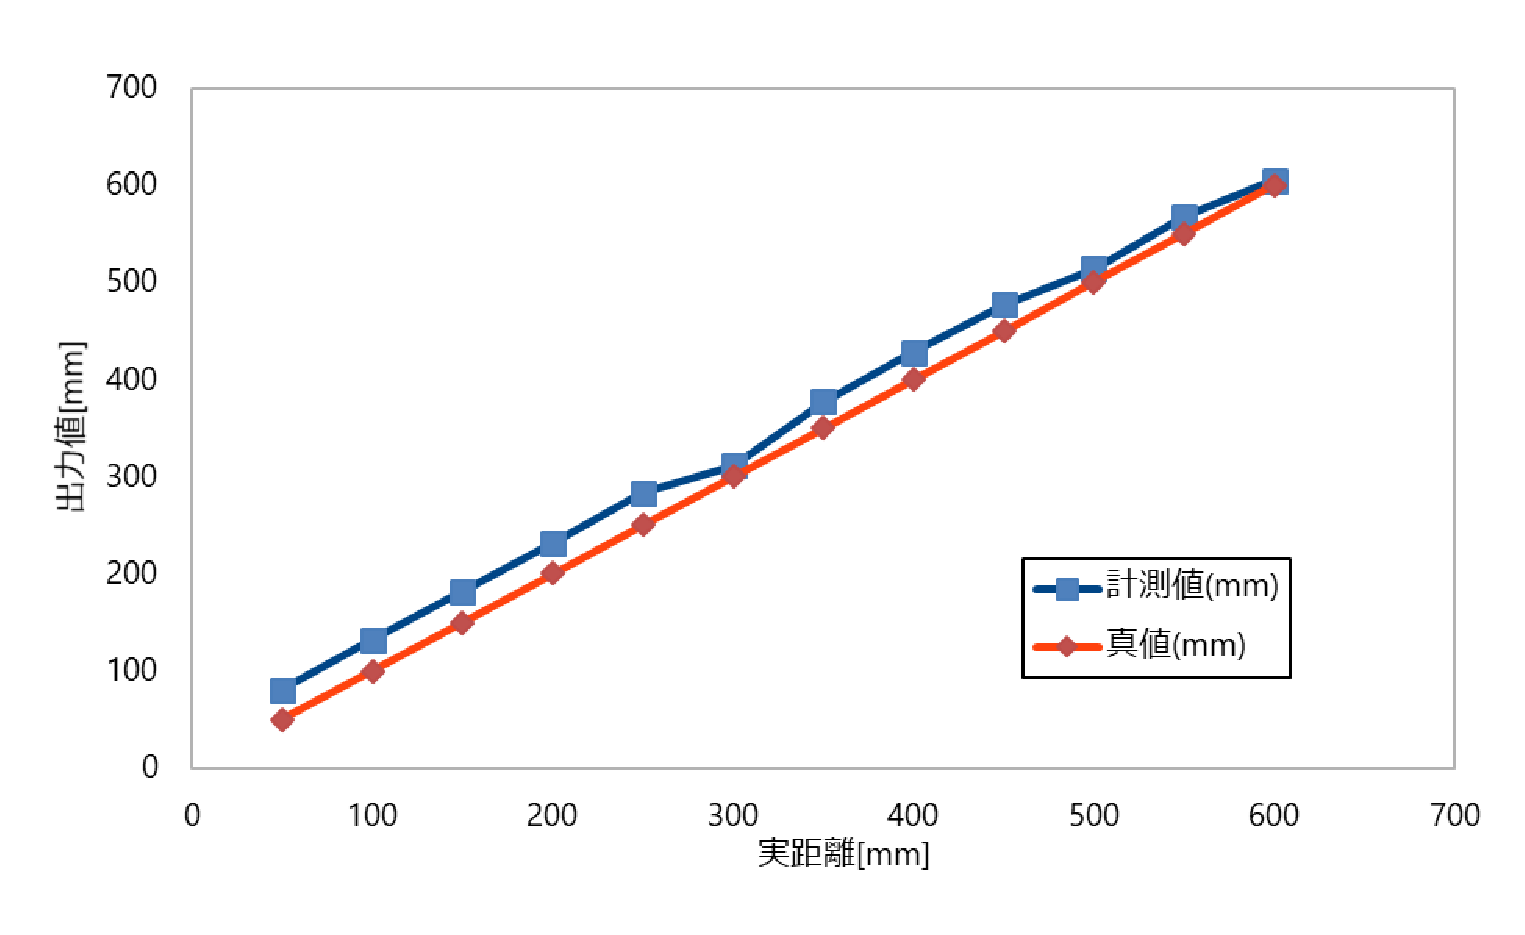
\includegraphics[width=0.5\hsize]{picture/eps/tof_sensor_experiment.eps}
  \caption{ToFセンサの特性}
  \label{fig::tof_graph}
 \end{figure}
